\documentclass{article}
\usepackage[a4paper,landscape,margin=0.72in]{geometry}
\usepackage{tikz}
\usetikzlibrary{calc,decorations.pathmorphing}

\pagestyle{empty}

\newcommand{\WTLx}{0.0}
\newcommand{\WTLy}{0.0}
\newcommand{\WBLx}{2.1}
\newcommand{\WBLy}{-5.7}
\newcommand{\WMx}{4.6}
\newcommand{\WMy}{-1.1}
\newcommand{\WBRx}{7.2}
\newcommand{\WBRy}{-5.9}
\newcommand{\WTRx}{9.8}
\newcommand{\WTRy}{0.0}
\newcommand{\WThreadWidth}{0.30pt}

\tikzset{
  pics/wfavorite/.style={
    code={
      \draw[line width=0.96pt,line cap=round,line join=round]
        (\WTLx pt,\WTLy pt)
        -- (\WBLx pt,\WBLy pt)
        -- (\WMx pt,\WMy pt)
        -- (\WBRx pt,\WBRy pt)
        -- (\WTRx pt,\WTRy pt);
    }
  },
  pics/wfavoritetrim/.style={
    code={
      \draw[line width=0.94pt,line cap=round,line join=round]
        (\WTLx pt,\WTLy pt)
        -- (1.9pt,-5.2pt)
        -- (4.1pt,-1.2pt)
        -- (6.8pt,-5.3pt)
        -- (\WTRx pt,-0.05pt);
    }
  },
  bosonleg/.style={
    line width=0.75pt,
    decorate,
    decoration={snake,amplitude=1.3mm,segment length=5.8mm}
  }
}

\newcommand{\DrawWUnits}[3]{%
  \foreach \i in {1,...,#1} {
    \pgfmathsetmacro{\SxTmp}{(\i-1)*#2}
    \pic at (\SxTmp pt,0pt) {#3};
  }
}

\newcommand{\DrawFootToTopChain}[5]{%
  \begin{scope}[shift={#1}, rotate=#2]
    \foreach \i in {1,...,#3} {
      \pgfmathtruncatemacro{\IsLastTmp}{ifthenelse(\i==#3,1,0)}
      \ifnum\IsLastTmp=0
        \pgfmathsetmacro{\SxTmp}{(\i-1)*#4}
        \pgfmathsetmacro{\NxTmp}{\i*#4}
        \draw[line width=\WThreadWidth,line cap=round]
          (\SxTmp pt+\WBRx pt,\WBRy pt) -- (\NxTmp pt+\WTLx pt,\WTLy pt);
      \fi
    }
    \DrawWUnits{#3}{#4}{#5}
  \end{scope}
}

\newcommand{\DrawBottomLeftToTopRightChain}[5]{%
  \begin{scope}[shift={#1}, rotate=#2]
    \foreach \i in {1,...,#3} {
      \pgfmathtruncatemacro{\IsLastTmp}{ifthenelse(\i==#3,1,0)}
      \ifnum\IsLastTmp=0
        \pgfmathsetmacro{\SxTmp}{(\i-1)*#4}
        \pgfmathsetmacro{\NxTmp}{\i*#4}
        \draw[line width=\WThreadWidth,line cap=round]
          (\SxTmp pt+\WBLx pt,\WBLy pt) -- (\NxTmp pt+\WTRx pt,\WTRy pt);
      \fi
    }
    \DrawWUnits{#3}{#4}{#5}
  \end{scope}
}

\newcommand{\DrawTopRightToBottomLeftChain}[5]{%
  \begin{scope}[shift={#1}, rotate=#2]
    \foreach \i in {1,...,#3} {
      \pgfmathtruncatemacro{\IsLastTmp}{ifthenelse(\i==#3,1,0)}
      \ifnum\IsLastTmp=0
        \pgfmathsetmacro{\SxTmp}{(\i-1)*#4}
        \pgfmathsetmacro{\NxTmp}{\i*#4}
        \draw[line width=\WThreadWidth,line cap=round]
          (\SxTmp pt+\WTRx pt,\WTRy pt) -- (\NxTmp pt+\WBLx pt,\WBLy pt);
      \fi
    }
    \DrawWUnits{#3}{#4}{#5}
  \end{scope}
}

\newcommand{\DrawAppliedFootToTop}[4]{%
  \path let \p1 = ($#2-#1$),
            \n1 = {veclen(\x1,\y1)/1pt},
            \n2 = {atan2(\y1,\x1)}
        in \pgfextra{\xdef\FitLenTmp{\n1}\xdef\FitAngTmp{\n2}};
  \pgfmathsetmacro{\FitRawLenTmp}{\FitLenTmp/#4}
  \pgfmathsetmacro{\FitAdvTmp}{(\FitRawLenTmp-\WTRx)/(#3-1)}
  \begin{scope}[shift={#1}, rotate=\FitAngTmp, scale=#4]
    \foreach \i in {1,...,#3} {
      \pgfmathtruncatemacro{\IsLastTmp}{ifthenelse(\i==#3,1,0)}
      \ifnum\IsLastTmp=0
        \pgfmathsetmacro{\SxTmp}{(\i-1)*\FitAdvTmp}
        \pgfmathsetmacro{\NxTmp}{\i*\FitAdvTmp}
        \draw[line width=\WThreadWidth/#4,line cap=round]
          (\SxTmp pt+\WBRx pt,\WBRy pt) -- (\NxTmp pt+\WTLx pt,\WTLy pt);
      \fi
    }
    \DrawWUnits{#3}{\FitAdvTmp}{wfavorite}
  \end{scope}
}

\newcommand{\DrawAppliedBottomLeftToTopRight}[4]{%
  \path let \p1 = ($#2-#1$),
            \n1 = {veclen(\x1,\y1)/1pt},
            \n2 = {atan2(\y1,\x1)}
        in \pgfextra{\xdef\FitLenTmp{\n1}\xdef\FitAngTmp{\n2}};
  \pgfmathsetmacro{\FitRawLenTmp}{\FitLenTmp/#4}
  \pgfmathsetmacro{\FitAdvTmp}{(\FitRawLenTmp-\WTRx)/(#3-1)}
  \begin{scope}[shift={#1}, rotate=\FitAngTmp, scale=#4]
    \foreach \i in {1,...,#3} {
      \pgfmathtruncatemacro{\IsLastTmp}{ifthenelse(\i==#3,1,0)}
      \ifnum\IsLastTmp=0
        \pgfmathsetmacro{\SxTmp}{(\i-1)*\FitAdvTmp}
        \pgfmathsetmacro{\NxTmp}{\i*\FitAdvTmp}
        \draw[line width=\WThreadWidth/#4,line cap=round]
          (\SxTmp pt+\WBLx pt,\WBLy pt) -- (\NxTmp pt+\WTRx pt,\WTRy pt);
      \fi
    }
    \DrawWUnits{#3}{\FitAdvTmp}{wfavorite}
  \end{scope}
}

\newcommand{\DrawAppliedTopRightToBottomLeft}[4]{%
  \path let \p1 = ($#2-#1$),
            \n1 = {veclen(\x1,\y1)/1pt},
            \n2 = {atan2(\y1,\x1)}
        in \pgfextra{\xdef\FitLenTmp{\n1}\xdef\FitAngTmp{\n2}};
  \pgfmathsetmacro{\FitRawLenTmp}{\FitLenTmp/#4}
  \pgfmathsetmacro{\FitAdvTmp}{(\FitRawLenTmp-\WTRx)/(#3-1)}
  \begin{scope}[shift={#1}, rotate=\FitAngTmp, scale=#4]
    \foreach \i in {1,...,#3} {
      \pgfmathtruncatemacro{\IsLastTmp}{ifthenelse(\i==#3,1,0)}
      \ifnum\IsLastTmp=0
        \pgfmathsetmacro{\SxTmp}{(\i-1)*\FitAdvTmp}
        \pgfmathsetmacro{\NxTmp}{\i*\FitAdvTmp}
        \draw[line width=\WThreadWidth/#4,line cap=round]
          (\SxTmp pt+\WTRx pt,\WTRy pt) -- (\NxTmp pt+\WBLx pt,\WBLy pt);
      \fi
    }
    \DrawWUnits{#3}{\FitAdvTmp}{wfavorite}
  \end{scope}
}

\begin{document}

\section*{W Propagator Favorites}

One compact artifact from the W-propagator exploration. These are the versions
worth keeping around: a clean uppercase-W chain, the literal lower-left to
next upper-right handoff, and the short layered bridge that stayed visually
promising in the applied vertex sketches.

\bigskip

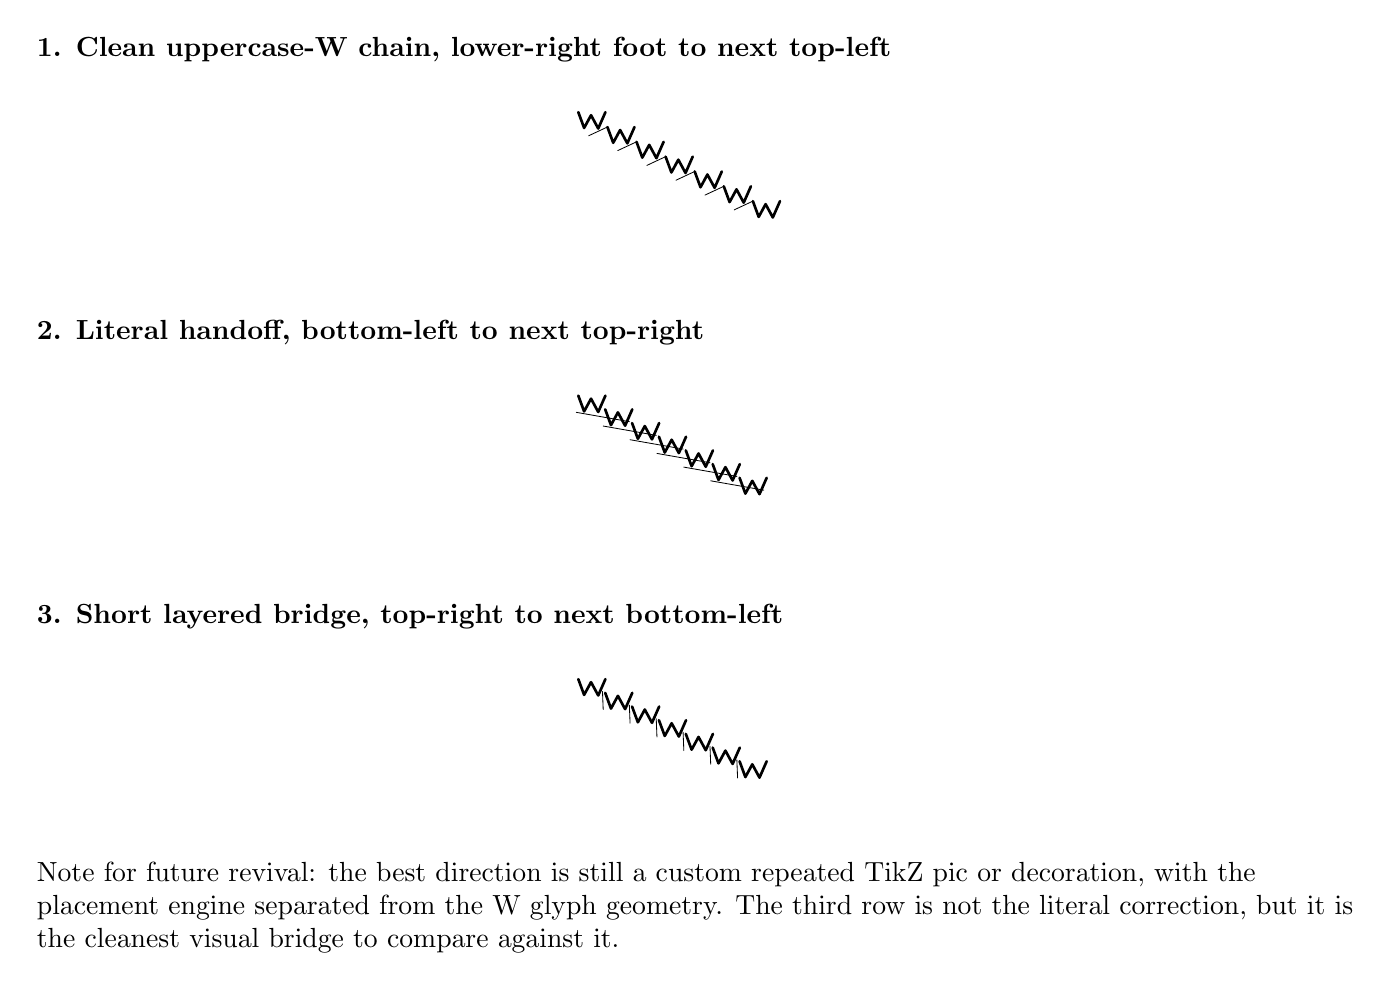
\begin{tikzpicture}[x=1cm,y=1cm]
  \node[anchor=west,font=\bfseries] at (0,11.9) {1. Clean uppercase-W chain, lower-right foot to next top-left};
  \DrawFootToTopChain{(7.0,11.1)}{-27}{7}{11.8}{wfavorite}

  \node[anchor=west,font=\bfseries] at (0,8.3) {2. Literal handoff, bottom-left to next top-right};
  \DrawBottomLeftToTopRightChain{(7.0,7.5)}{-27}{7}{10.9}{wfavorite}

  \node[anchor=west,font=\bfseries] at (0,4.7) {3. Short layered bridge, top-right to next bottom-left};
  \DrawTopRightToBottomLeftChain{(7.0,3.9)}{-27}{7}{10.9}{wfavorite}

  \node[align=flush left,anchor=west,text width=16.8cm] at (0,1.0) {%
    Note for future revival: the best direction is still a custom repeated
    TikZ pic or decoration, with the placement engine separated from the W
    glyph geometry. The third row is not the literal correction, but it is the
    cleanest visual bridge to compare against it.};
\end{tikzpicture}

\newpage

\section*{Applied 3-Point Geometry}

\begin{tikzpicture}[x=1cm,y=1cm]
  \node[anchor=west,font=\bfseries] at (0,12.4) {1. Foot-to-top chain};
  \node[anchor=west,font=\bfseries] at (6.5,12.4) {2. Literal handoff};
  \node[anchor=west,font=\bfseries] at (13.0,12.4) {3. Layered bridge};

  \coordinate (A) at (3.1,7.8);
  \coordinate (AUL) at (0.8,10.7);
  \coordinate (AR) at (5.4,7.8);
  \coordinate (AB) at (3.1,4.5);
  \fill (A) circle[radius=2.6pt];
  \DrawAppliedFootToTop{(AUL)}{(A)}{7}{1.02}
  \draw[bosonleg] (A) -- (AR);
  \draw[bosonleg] (A) -- (AB);

  \coordinate (B) at (9.6,7.8);
  \coordinate (BUL) at (7.3,10.7);
  \coordinate (BR) at (11.9,7.8);
  \coordinate (BB) at (9.6,4.5);
  \fill (B) circle[radius=2.6pt];
  \DrawAppliedBottomLeftToTopRight{(BUL)}{(B)}{7}{1.02}
  \draw[bosonleg] (B) -- (BR);
  \draw[bosonleg] (B) -- (BB);

  \coordinate (C) at (16.1,7.8);
  \coordinate (CUL) at (13.8,10.7);
  \coordinate (CR) at (18.4,7.8);
  \coordinate (CB) at (16.1,4.5);
  \fill (C) circle[radius=2.6pt];
  \DrawAppliedTopRightToBottomLeft{(CUL)}{(C)}{7}{1.02}
  \draw[bosonleg] (C) -- (CR);
  \draw[bosonleg] (C) -- (CB);

  \node[anchor=south east] at (AUL) {$W_1$};
  \node[anchor=west] at (AR) {$A_2$};
  \node[anchor=north] at (AB) {$A_3$};
  \node[anchor=south east] at (BUL) {$W_1$};
  \node[anchor=west] at (BR) {$A_2$};
  \node[anchor=north] at (BB) {$A_3$};
  \node[anchor=south east] at (CUL) {$W_1$};
  \node[anchor=west] at (CR) {$A_2$};
  \node[anchor=north] at (CB) {$A_3$};
\end{tikzpicture}

\end{document}
